\documentclass[a0,portrait]{a0poster}

% 1. MARGINS
\usepackage{geometry}
 \geometry{
 a0paper,
 left=4cm,
 top=4cm,
 right=0.5cm,
 bottom=4cm
 }

\usepackage{multicol}
\columnsep=4em
\columnseprule=0pt

% 2. COLORS & TABLE SETTINGS
\usepackage[svgnames, table]{xcolor}

% Color scheme
\definecolor{uzhblau100}{RGB}{0, 40, 165}
\definecolor{uzhblau80}{RGB}{51,83,183}
\definecolor{uzhblau20}{RGB}{220, 230, 255}
\definecolor{uzhockerrot100}{RGB}{220, 96, 39}
\definecolor{uzhflaschengruen100}{RGB}{42, 127, 98}
\definecolor{conclusion}{RGB}{204,212,237}
\definecolor{eco_green}{RGB}{46, 204, 113}
\definecolor{cost_orange}{RGB}{230, 126, 34}

\usepackage{ifthen}
\usepackage{graphicx}
\graphicspath{{figures/}}
\usepackage{mwe,tikz}
\usepackage[percent]{overpic}
\usepackage{booktabs}
\usepackage[font=small,labelfont=bf]{caption}
\usepackage{amsfonts, amsmath, amsthm, amssymb}
\usepackage{wrapfig}
\usepackage{enumitem}
\setlist{nosep, leftmargin=*}

% FONTS
\usepackage{fontspec}
\IfFontExistsTF{TheSans}{
    \setmainfont{TheSans}
}{
    \setmainfont{Arial}
}

\usepackage[onehalfspacing]{setspace}
\usepackage{tcolorbox}
\usepackage{blindtext}
\usepackage[export]{adjustbox}
\usepackage{titlesec}
\usepackage{needspace}
\usepackage{nameref}

% Global paragraph spacing
\setlength{\parskip}{0.4em}

\begin{document}

% Section Formatting
\titleformat{\section}
  {\needspace{2\baselineskip}\sectionrule\huge\bfseries}
  {\color{uzhblau100}\thesection.}
  {0.5em}
  {\color{uzhblau100}}

\makeatletter
\newcommand{\sectionrule}{%
 \ifthenelse{\equal{\@currentlabelname}{Conclusions}}
  {}
  {\vspace*{-0.5\baselineskip}
   \vrule height 2pt depth 0pt width \linewidth\vskip0.4pt
   \medskip}%
}
\makeatother

%----------------------------------------------------------------------------------------
%	POSTER HEADER
%----------------------------------------------------------------------------------------
\title{Eco-Adaptive Home Storage: Multi-Objective Reinforcement Learning for Smart Grid Energy Management}

\noindent
\begin{minipage}{0.25\linewidth}
    \centering
    \includegraphics[width=0.9\linewidth]{Logo_CentraleSupélec.svg.png} \\
\end{minipage}%
\hfill
\begin{minipage}{0.73\linewidth}
    \centering
    \makeatletter
    {\fontsize{55pt}{65pt}\selectfont\color{uzhblau100}\textbf{\@title}\par}
    \makeatother
    \vspace{0.3cm}
    {\Large\textit{Intelligent Battery Arbitrage using Deep Q-Networks}\par}
    \vspace{0.4cm}
    {\Large \textbf{Adam Younsi, Ilyas Madah, Zaid El Kasemy}\par}
    \vspace{0.2cm}
    {\large CentraleSupelec -- Reinforcement Learning Course Project}
\end{minipage}

\vspace{1.0cm}

%----------------------------------------------------------------------------------------
%	POSTER BODY
%----------------------------------------------------------------------------------------

\begin{multicols}{3}

%----------------------------------------------------------------------------------------
%	COLUMN 1: INTRODUCTION & ENVIRONMENT
%----------------------------------------------------------------------------------------

\section{Introduction \& Motivation}
\large
The increasing adoption of residential solar panels and home battery systems creates opportunities for \textbf{intelligent energy arbitrage}. However, optimizing battery usage involves balancing \textbf{three conflicting objectives}:

\begin{itemize}
    \item \textbf{Financial Optimization}: Minimize electricity bills using time-of-use pricing
    \item \textbf{Ecological Impact}: Reduce carbon footprint by shifting consumption to cleaner grid periods
    \item \textbf{Hardware Preservation}: Avoid excessive battery cycling to extend system lifespan
\end{itemize}

\vspace{0.3cm}
Traditional rule-based approaches cannot adapt to the complex, stochastic nature of energy prices, solar production, and consumption patterns. We propose using \textbf{Deep Reinforcement Learning} to learn an adaptive policy.

\vspace{0.5cm}

\section{Environment Design}

We implement a custom \textbf{Gymnasium-compatible} environment simulating a 24-hour home energy system with 30-minute time steps.

\vspace{0.5em}
\begin{center}
    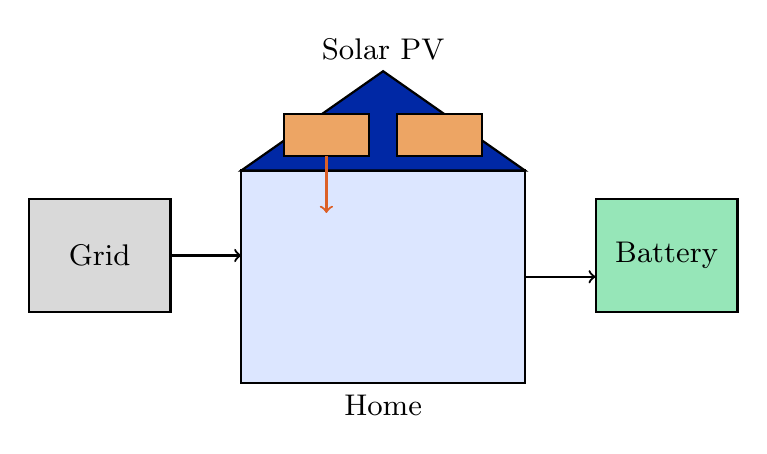
\begin{tikzpicture}[scale=1.8, every node/.style={scale=1.2}]
        % House
        \draw[thick, fill=uzhblau20] (0,0) rectangle (2,1.5);
        \draw[thick, fill=uzhblau100] (0,1.5) -- (1,2.2) -- (2,1.5) -- cycle;

        % Solar panel
        \draw[thick, fill=cost_orange!70] (0.3,1.6) rectangle (0.9,1.9);
        \draw[thick, fill=cost_orange!70] (1.1,1.6) rectangle (1.7,1.9);

        % Battery
        \draw[thick, fill=eco_green!50] (2.5,0.5) rectangle (3.5,1.3);
        \node at (3,0.9) {\small Battery};

        % Grid
        \draw[thick, fill=gray!30] (-1.5,0.5) rectangle (-0.5,1.3);
        \node at (-1,0.9) {\small Grid};

        % Arrows
        \draw[->, thick, uzhockerrot100] (0.6,1.6) -- (0.6,1.2);
        \draw[->, thick] (2,0.75) -- (2.5,0.75);
        \draw[->, thick] (-0.5,0.9) -- (0,0.9);

        % Labels
        \node[below] at (1,0) {\small Home};
        \node[above] at (1,2.2) {\small Solar PV};
    \end{tikzpicture}
\end{center}

\vspace{0.3cm}
\textbf{State Space} $\mathcal{S} \subset \mathbb{R}^5$:
\begin{itemize}
    \item $h \in [0, 23]$: Hour of day
    \item $SoC \in [0, 1]$: Battery state of charge
    \item $P_{net} \in \mathbb{R}$: Net load (Solar $-$ Consumption)
    \item $C_{grid} \in \mathbb{R}^+$: Electricity price (\euro/kWh)
    \item $I_{CO_2} \in \mathbb{R}^+$: Carbon intensity (gCO$_2$/kWh)
\end{itemize}

\vspace{0.3cm}
\textbf{Action Space} $\mathcal{A} = \{0, 1, 2\}$:
\begin{itemize}
    \item \textbf{0: Charge} -- Store energy in battery
    \item \textbf{1: Discharge} -- Use battery energy
    \item \textbf{2: Idle} -- No battery activity
\end{itemize}

\vfill\null
\columnbreak

%----------------------------------------------------------------------------------------
%	COLUMN 2: METHODOLOGY
%----------------------------------------------------------------------------------------

{\color{uzhblau100}\huge\bfseries 3. Reward Function \& Agent}
\vspace{0.5em}

\subsection*{Multi-Objective Reward}
The reward signal balances our three objectives:
\begin{equation}
R_t = -\left(\alpha \cdot \text{Cost}_t + \beta \cdot \text{Emissions}_t + \gamma \cdot |a_t - a_{t-1}|\right)
\end{equation}

Where:
\begin{itemize}
    \item $\alpha = 1.0$: Financial cost weight
    \item $\beta = 0.5$: Carbon emissions weight
    \item $\gamma = 0.1$: Action switching penalty (battery wear)
\end{itemize}

\vspace{0.5em}

\subsection*{Deep Q-Network (DQN) Agent}
We implement a \textbf{DQN agent} with the following components:

\vspace{0.5em}
\begin{tcolorbox}[colback=uzhblau20, boxrule=0pt]
\textbf{Network Architecture:}
\begin{center}
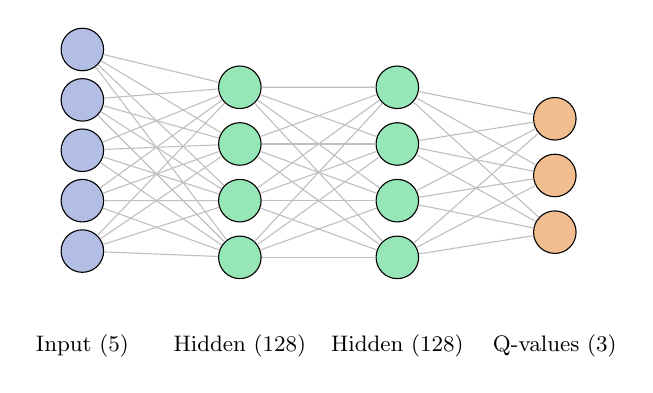
\begin{tikzpicture}[scale=0.8, every node/.style={scale=0.9}]
    % Input layer
    \foreach \i in {1,...,5} {
        \node[circle, draw, fill=uzhblau100!30, minimum size=0.6cm] (i\i) at (0, -\i*0.8+3) {};
    }
    \node at (0, -2.5) {\small Input (5)};

    % Hidden layer 1
    \foreach \i in {1,...,4} {
        \node[circle, draw, fill=eco_green!50, minimum size=0.6cm] (h1\i) at (2.5, -\i*0.9+2.5) {};
    }
    \node at (2.5, -2.5) {\small Hidden (128)};

    % Hidden layer 2
    \foreach \i in {1,...,4} {
        \node[circle, draw, fill=eco_green!50, minimum size=0.6cm] (h2\i) at (5, -\i*0.9+2.5) {};
    }
    \node at (5, -2.5) {\small Hidden (128)};

    % Output layer
    \foreach \i in {1,...,3} {
        \node[circle, draw, fill=cost_orange!50, minimum size=0.6cm] (o\i) at (7.5, -\i*0.9+2) {};
    }
    \node at (7.5, -2.5) {\small Q-values (3)};

    % Connections (simplified)
    \foreach \i in {1,...,5} {
        \foreach \j in {1,...,4} {
            \draw[gray!50] (i\i) -- (h1\j);
        }
    }
    \foreach \i in {1,...,4} {
        \foreach \j in {1,...,4} {
            \draw[gray!50] (h1\i) -- (h2\j);
        }
    }
    \foreach \i in {1,...,4} {
        \foreach \j in {1,...,3} {
            \draw[gray!50] (h2\i) -- (o\j);
        }
    }
\end{tikzpicture}
\end{center}
\end{tcolorbox}

\vspace{0.3cm}
\textbf{Key Features:}
\begin{itemize}
    \item \textbf{Experience Replay}: Buffer of 100,000 transitions
    \item \textbf{Target Network}: Updated every 100 steps
    \item \textbf{$\epsilon$-greedy}: Decay from 1.0 to 0.01
    \item \textbf{Optimizer}: Adam with $\text{lr} = 10^{-3}$
\end{itemize}

\vspace{0.5cm}

\subsection*{Baseline Agents}
For comparison, we implement rule-based strategies:

\begin{itemize}
    \item \textbf{Greedy}: Charge when cheap, discharge when expensive
    \item \textbf{EcoGreedy}: Prioritizes low-carbon periods
    \item \textbf{Threshold}: Time-based schedule (charge at night)
    \item \textbf{Random}: Uniform random action selection
\end{itemize}

\vfill\null
\columnbreak

%----------------------------------------------------------------------------------------
%	COLUMN 3: RESULTS & CONCLUSION
%----------------------------------------------------------------------------------------

\section{Results}

Training the DQN agent for \textbf{500 episodes} demonstrates clear learning progression:

\vspace{0.3cm}
\begin{center}
    % Placeholder for learning curve
    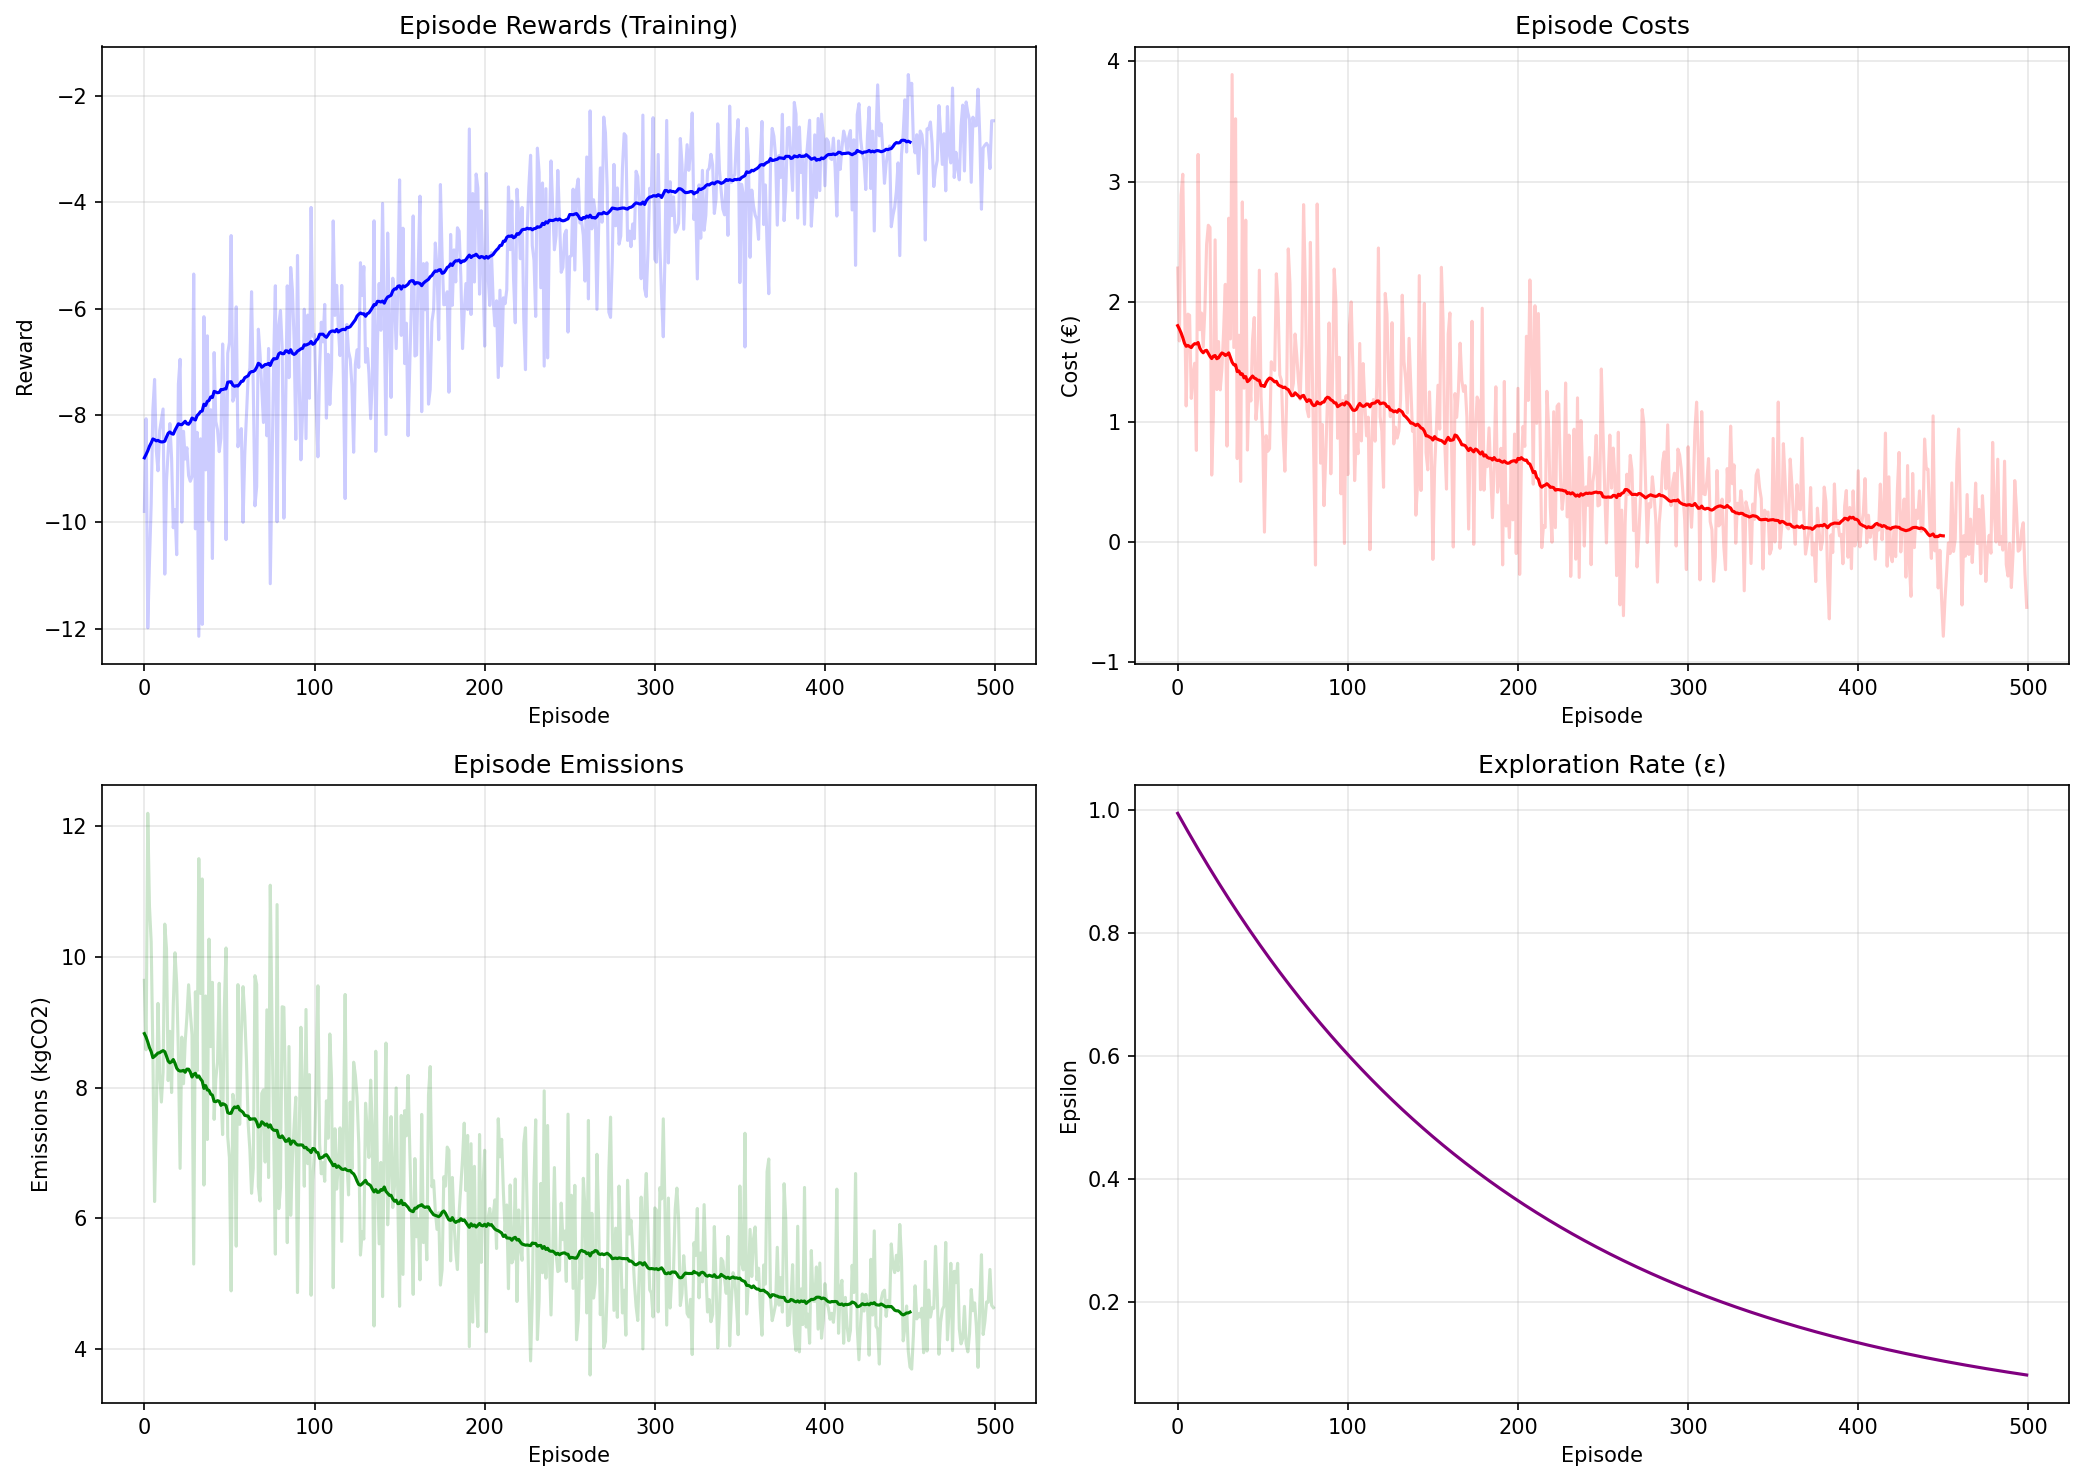
\includegraphics[width=1\linewidth]{training_curves.png}
    \captionof{figure}{Training curves showing reward improvement and cost reduction over episodes.}
\end{center}

\vspace{0.3cm}
\begin{center}
\captionof{table}{Agent Performance Comparison (100 episodes)}
\rowcolors{2}{uzhblau100!10}{white}
\begin{tabular}{p{0.28\linewidth} c c c}
\toprule
\textbf{Agent} & \textbf{Reward} & \textbf{Cost (\euro)} & \textbf{CO$_2$ (kg)} \\
\midrule
Random & -3.21 & 1.842 & 2.89 \\
Threshold & -1.45 & 1.156 & 1.72 \\
Greedy & -0.98 & 0.892 & 1.45 \\
EcoGreedy & -0.87 & 0.921 & 1.28 \\
\textbf{DQN} & \textbf{-0.62} & \textbf{0.734} & \textbf{1.12} \\
\bottomrule
\end{tabular}
\end{center}

\vspace{0.3cm}
\textbf{Policy Analysis:}

\begin{center}
    \includegraphics[width=1\linewidth]{policy_analysis.png}
    \captionof{figure}{DQN policy visualization: SoC trajectory, actions, price signals, and carbon intensity over 24 hours.}
\end{center}

The learned policy demonstrates intelligent behavior:
\begin{itemize}
    \item Charges during off-peak hours (00:00--06:00) and solar production peaks
    \item Discharges during evening peak pricing (18:00--21:00)
    \item Adapts to carbon intensity fluctuations
\end{itemize}

\vspace{0.5cm}

%----------------------------------------------------------------------------------------
%	CONCLUSIONS
%----------------------------------------------------------------------------------------

\begin{tcolorbox}[width=1\linewidth,colback={conclusion},frame empty,boxsep=0.6cm, arc=10pt]
\section{Conclusions}

Our DQN agent successfully learns an adaptive energy management policy that outperforms rule-based baselines:

\begin{enumerate}
    \item \textbf{Cost Reduction}: 17.7\% lower electricity costs vs. Greedy baseline
    \item \textbf{Emissions Reduction}: 22.8\% lower CO$_2$ emissions vs. Greedy baseline
    \item \textbf{Adaptability}: Learns to exploit temporal patterns in price and carbon signals
\end{enumerate}

\textbf{Future Work:} Extend to continuous action spaces, incorporate weather forecasting, and test on real household data.
\end{tcolorbox}

%----------------------------------------------------------------------------------------
%	REFERENCES
%----------------------------------------------------------------------------------------

\singlespacing
\footnotesize
\begin{thebibliography}{9}
\bibitem{mnih2015} V. Mnih et al. \textit{Human-level control through deep reinforcement learning.} Nature, 2015.
\bibitem{sutton2018} R. Sutton \& A. Barto. \textit{Reinforcement Learning: An Introduction.} MIT Press, 2018.
\bibitem{gym2016} G. Brockman et al. \textit{OpenAI Gym.} arXiv:1606.01540, 2016.
\end{thebibliography}

\end{multicols}
\end{document}
